\section{Выполнение работы}
\subsection{Описание предметной области}
В лаборатории работают ученые.
Ученые могут участвовать в переговорах.
Ученые могут владеть фондами.
Ученые могут совершать действия.
Действия могут совершаться как без субъекта, так и с субъектом.
Действия могут совершаться как на переговорах, так и не на переговорах.

В лаборатории также существуют животные.
Ученые разрабатывают животных.
У каждого животного есть как минимум один создатель.
Животные находятся в клетке, клетка может быть похожа на какую-то вещь.
Клетка также может бьть покрыта какой-либо вещью.


\subsection{Список сущностей и их классификация}
\begin{itemize}
  \item Стержневые сущности:
        \begin{itemize}
          \item Ученый (имя)
          \item Существо (название)
          \item Клетка (хранимое животное)
          \item Вещь (описание)
          \item Фонд (владелец)
          \item Переговоры (время проведения)
          \item Действия (описание)
        \end{itemize}

  \item Ассоциативные:
        \begin{itemize}
          \item Связь ученые --- существа отражает создателей существа
          \item Связь ученые --- действия отражает действия, совершенные ученым
          \item Связь действие --- клетка отражает объект действия
          \item Связь действие --- вещи отражает объект действия
          \item Связь действие --- переговоры отражает на каких переговорах было совершено действие
          \item Связь клетка --- вещь отражает схожесть клетки с вещью
          \item Связь ученые --- переговоры отражает участие ученого в переговорах
        \end{itemize}

  \item Характеристические:
        \begin{itemize}
          \item Связь клетка --- существо отражает нахождение существа в клетке
          \item Связь фонд --- ученый отражает владение фондом
          \item Связь клетка --- вещь отражает накрытие клетки вещью
          \item Связь действие --- клетка отражает субъект действия
          \item Связь действие --- вещь отражает субъект действия
        \end{itemize}
\end{itemize}


\begin{figure}[ht]
  \centering
  % 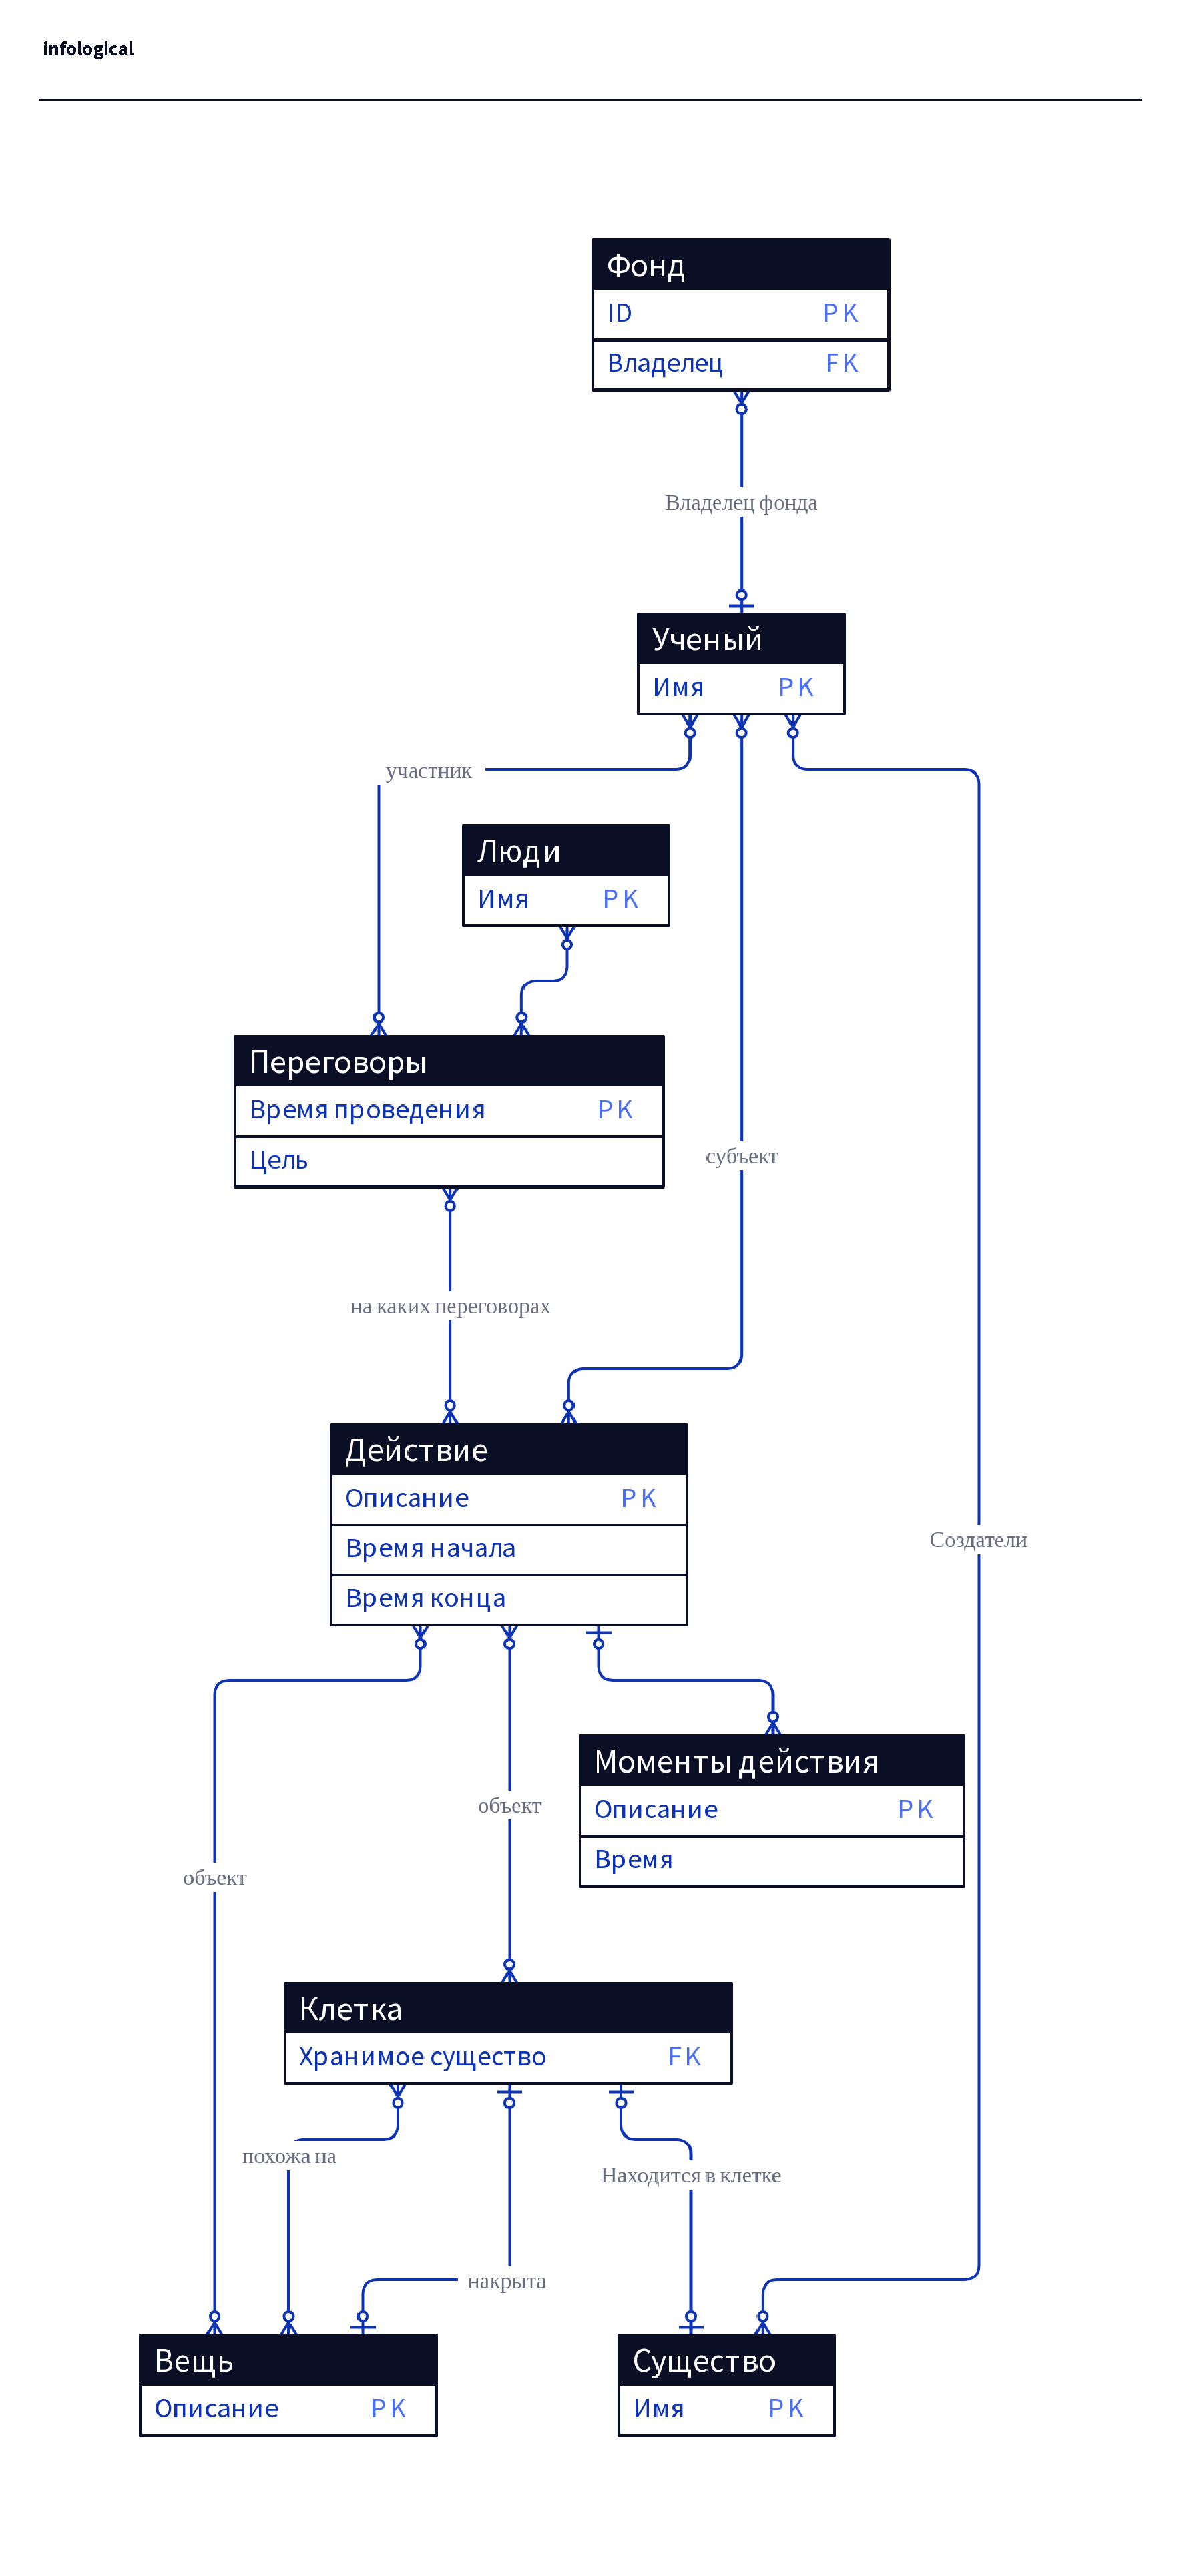
\includegraphics[width=\textwidth]{img/infological.pdf}
  \resizebox{0.9\textwidth}{!}{
  \input{../out/plantuml/infological/infological.latex}
  }
  \caption{Инфологическая модель}
\end{figure}


\clearpage
\begin{figure}[ht]
  \centering
    \resizebox{0.9\textwidth}{!}{
  \input{../out/plantuml/datalogical/datalogical.latex}
  }
  \caption{Даталогическая модель}
\end{figure}

\subsection{Реализация модели на SQL}

\inputminted[breaklines]{SQL}{../scheme.sql}
